\documentclass[11pt]{article}

\usepackage[margin=1in]{geometry}
\usepackage{amsmath,amssymb}
\usepackage{booktabs}
\usepackage{graphicx}
\usepackage{microtype}
\usepackage{xcolor}
\usepackage{hyperref}

\hypersetup{
  colorlinks=true,
  linkcolor=blue!55!black,
  citecolor=blue!55!black,
  urlcolor=blue!55!black
}

\newcommand{\logit}{\operatorname{logit}}
\newcommand{\pred}{\mathrm{pred}}
\newcommand{\act}{\mathrm{act}}

\title{Can Language Models Forecast Their Own Belief Updates?\\
\large A Two-Context Test of Metacognitive Forecast Revision}
\author{Invariant Forecasting Project}
\date{\today}

\begin{document}
\maketitle

\begin{abstract}
Probabilistic forecasts are useful only insofar as they can be revised under
new evidence. Recent work studies whether language models can forecast future
events, whether they update beliefs in a Bayes-like manner, and whether they
can predict aspects of their own future behavior. We connect these threads with
a direct metacognitive test: can a language model predict how its own forecast
will change after seeing evidence? For each forecasting question $X$ and
neutral evidence packet $Y$, we first elicit the model's current probability
$\pi=P(X)$. In the same context, before allowing an ordinary update, we ask the
model to predict what its own posterior would be after receiving $Y$. In a
fresh context, we then actually provide $Y$ and elicit the realized posterior.
We compare predicted and realized updates in log-odds space. On the full 343-question
ForecastBench-derived validation split using GPT-OSS-120B, the model's predicted
and realized log-odds updates have Spearman correlation $0.908$ and Pearson
correlation $0.894$, reducing mean absolute log-odds error by $65.4\%$
relative to a no-update baseline. The result is stable under robustness checks:
restricting to $|\Delta_{\act}|<5$ gives Spearman $0.907$ and Pearson $0.886$.
Error analysis shows that failures are concentrated in a small number of
near-boundary probability cases, while ordinary-sized updates are strongly
predictable. These results
suggest that language models exhibit measurable self-forecasting of their own
evidence-conditioned forecast revisions, without implying Bayes optimality or
privileged access to internal beliefs.
\end{abstract}

\section{Introduction}

Forecasting systems should not merely issue probabilities; they should also
revise them coherently when new information arrives. Large language models
(LLMs) are increasingly evaluated as forecasters on real-world questions
\cite{halawi2024forecasting,karger2024forecastbench}. Separately, a growing
literature asks whether LLMs can evaluate their own knowledge or anticipate
their own behavior \cite{kadavath2022know,ashok2025behavior,binder2024inward},
and another asks whether LLMs can perform probabilistic or Bayesian-style
belief updating \cite{qiu2026bayesian}. What is missing is the direct bridge:
can a model predict its own future belief update before the evidence is
actually shown in an ordinary forecasting context?

We propose a simple two-context protocol. Given a binary question $X$, first
elicit the model's current forecast $\pi$. Then, in the same context, present a
counterfactual description of evidence $Y$ and ask the model to predict the
posterior it would give after incorporating $Y$. Finally, in a fresh context,
provide the same evidence $Y$ and elicit the model's actual posterior. The
central object is not the posterior itself, but the update:
\begin{align}
  \Delta_{\pred} &= \logit(\pi'_{\pred}) - \logit(\pi),\\
  \Delta_{\act} &= \logit(\pi'_{\act}) - \logit(\pi).
\end{align}
If models have metacognitive access to their own forecast revision behavior,
then $\Delta_{\pred}$ should track $\Delta_{\act}$ across many $(X,Y)$ pairs.

This paper reports an initial, deliberately narrow result: neutral evidence
packets only, one model, and the full 343-question validation split. The result is nonetheless
sharp. Predicted and actual updates are strongly rank-correlated, substantially
closer than a no-update baseline, and robust after excluding exact boundary
probabilities. The remaining failures are also interpretable: they are mostly near-boundary
probability cases or directional disagreements on individual questions, rather
than a broad collapse of self-prediction.

\section{Protocol}

Each example consists of a binary forecasting question $X$, a prior phase, and
a neutral evidence packet $Y$ dated before the forecast date. The prior phase
includes the question, source background, resolution criteria, forecast date,
resolution date, and a reference-class base rate. The base rate is shown as
context, but in the exact protocol it is not used as $\pi$; $\pi$ is elicited
from the model.

\paragraph{Step 1: elicit the current forecast.}
The model receives only the prior phase and is asked to output a probability on
the first line in the form \texttt{Probability: <number between 0 and 1>}. This
probability is $\pi$.

\paragraph{Step 2: predict the future update.}
In the same conversation, the model is told that it is about to receive evidence
$Y$ in a separate ordinary forecast. Before making that ordinary forecast, it is
asked to predict what its own posterior forecast would become after
incorporating $Y$. This yields $\pi'_{\pred}$.

\paragraph{Step 3: realize the update in a fresh context.}
In a new context, the model receives the same prior phase, acknowledges that it
will use the prior phase as its starting point, then receives $Y$ as the update
phase and outputs a posterior. This yields $\pi'_{\act}$.

\paragraph{Metric.}
We compare log-odds updates from the same elicited prior. To avoid infinite
values, probabilities are clipped to $[10^{-6},1-10^{-6}]$ before applying
$\logit(p)=\log(p/(1-p))$. We report Pearson and Spearman correlations between
$\Delta_{\pred}$ and $\Delta_{\act}$, mean absolute error (MAE), RMSE, posterior
probability gap, and improvement over a no-update baseline
($\Delta_{\pred}=0$).

\section{Data and Model}

We evaluate on all 343 validation questions from the repository's
ForecastBench-derived dataset. The evidence packets are the neutral variants of
the generated prior/update dataset; stronger weak-yes, strong-yes, weak-no, and
strong-no framings are reserved for future experiments. We run GPT-OSS-120B via
Tinker sampling at temperature $0$, top-$p=1$, and a 512-token generation cap.
The run produced 342 parseable prior forecasts and 330 fully parseable
prior/predicted/actual triples, giving pair coverage $96.2\%$.

\section{Results}

\begin{table}[t]
\centering
\small
\begin{tabular}{lrrr}
\toprule
Metric & All rows & Excl. exact 0/1 & $|\Delta_{\act}|<5$ \\
\midrule
Parseable pairs / rows & 330 / 343 & 330 / 343 & 329 / 343 \\
Pearson corr. & 0.894 & 0.894 & 0.886 \\
Spearman corr. & 0.908 & 0.908 & 0.907 \\
Log-odds MAE & 0.289 & 0.289 & 0.290 \\
Log-odds RMSE & 0.438 & 0.438 & 0.438 \\
Posterior RMSE & 0.041 & 0.041 & 0.041 \\
No-update MAE & 0.836 & 0.836 & 0.824 \\
MAE improvement vs no-update & 65.4\% & 65.4\% & 64.8\% \\
\bottomrule
\end{tabular}
\caption{Main exact-protocol results. The model substantially predicts its own
future update. Boundary filtering and a $|\Delta_{\act}|<5$ restriction leave
the main conclusion essentially unchanged.}
\label{tab:main}
\end{table}

Table~\ref{tab:main} gives the main result. Across all parseable pairs,
predicted and actual log-odds shifts have Spearman correlation $0.908$ and
Pearson correlation $0.894$. The model reduces log-odds MAE by $65.4\%$
relative to predicting no update. Unlike the earlier 200-group smoke test, the
full validation run contains no exact $0/1$ posteriors among parseable pairs, so
the all-row and boundary-filtered metrics coincide. Restricting to
$|\Delta_{\act}|<5$ yields nearly identical results.

\begin{figure}[t]
\centering
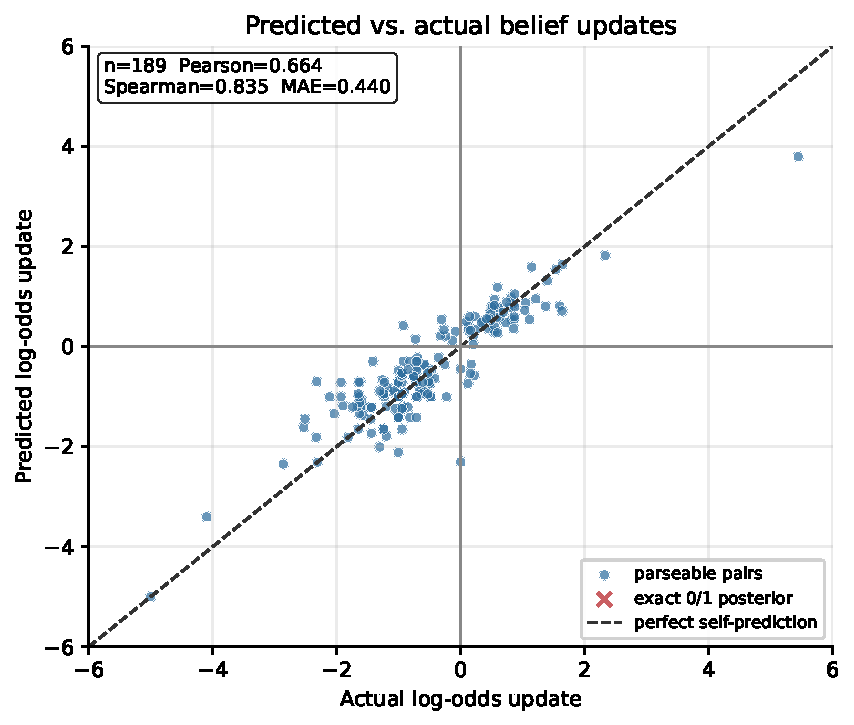
\includegraphics[width=0.72\linewidth]{figures/predicted_vs_actual_updates.pdf}
\caption{Predicted versus actual log-odds updates in the exact two-context
protocol. The dashed line is perfect self-prediction.}
\label{fig:scatter}
\end{figure}

Figure~\ref{fig:scatter} shows the same pattern visually. Most points cluster
around the diagonal, with no exact $0/1$ posterior among parseable pairs in the
full validation run.

\section{Distribution-Conditional Diagnostics}

The full validation run supports a distribution-conditional story: the model
predicts ordinary updates especially well, while rare extreme updates are too
few to estimate reliably. We therefore
condition on $|\Delta_{\act}|$ bins.

\begin{table}[t]
\centering
\small
\begin{tabular}{lrrrrrr}
\toprule
$|\Delta_{\act}|$ bin & $n$ & Pearson & Spearman & MAE & RMSE & Post. MAE \\
\midrule
$<1$ & 229 & 0.874 & 0.885 & 0.205 & 0.311 & 0.025 \\
$[1,3)$ & 99 & 0.848 & 0.701 & 0.476 & 0.629 & 0.017 \\
$[3,5)$ & 1 & -- & -- & 1.386 & 1.386 & 0.00015 \\
$\geq5$ & 1 & -- & -- & 0.000 & 0.000 & 0.000 \\
\bottomrule
\end{tabular}
\caption{Performance conditioned on actual update extremity. Most examples
fall below $|\Delta_{\act}|<3$, where linear/rank correlations and errors
remain strong. The extreme bins are too small for stable correlation estimates.}
\label{tab:bins}
\end{table}

\begin{figure}[t]
\centering
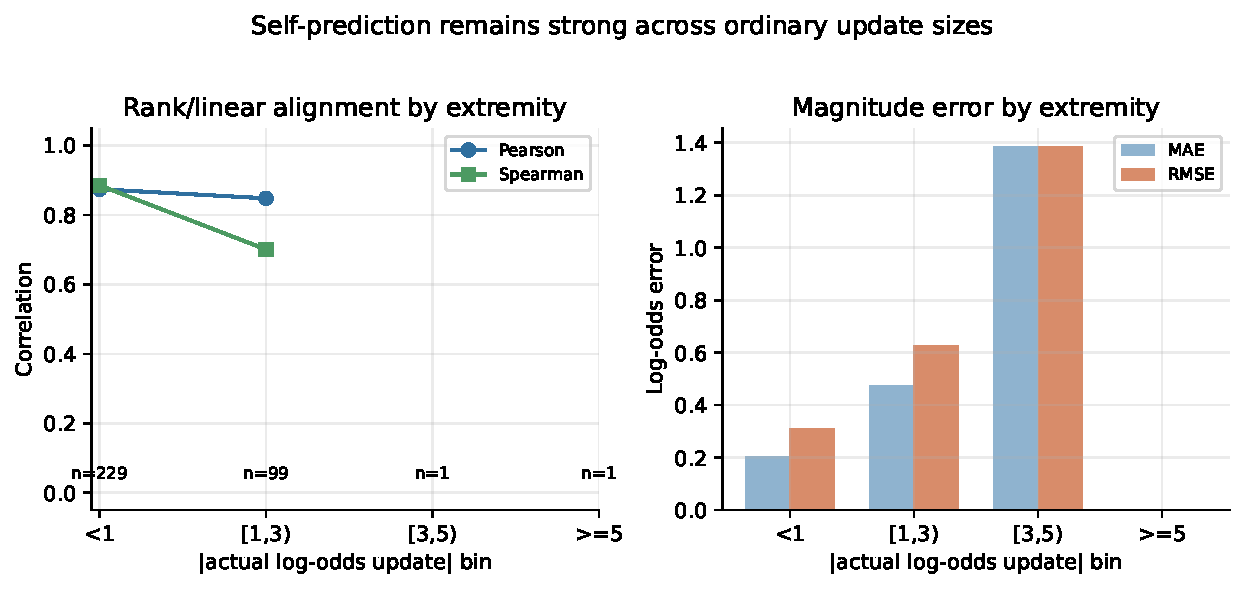
\includegraphics[width=0.88\linewidth]{figures/extremity_bins.pdf}
\caption{Correlations and error by actual-update extremity. The two-regime
picture is visible: ordinary updates are predictable; rare extreme shifts are
sparse in this validation split.}
\label{fig:bins}
\end{figure}

\begin{figure}[t]
\centering
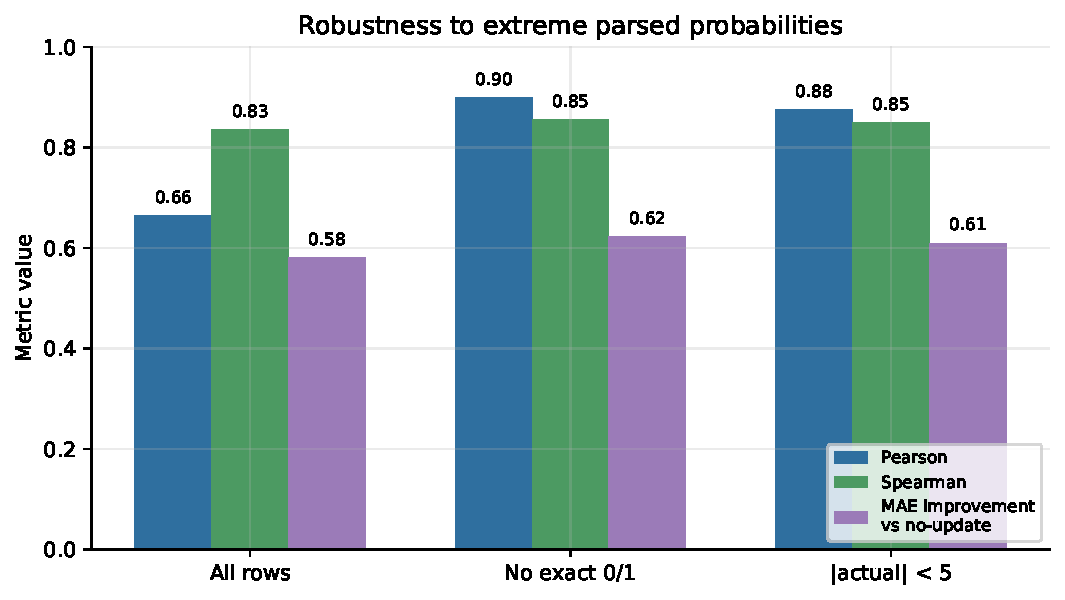
\includegraphics[width=0.78\linewidth]{figures/robustness_summary.pdf}
\caption{Robustness of the headline metrics. Boundary filtering leaves the full-validation result unchanged, while
restricting to $|\Delta_{\act}|<5$ preserves high Pearson/Spearman correlation
and large improvement over no-update.}
\label{fig:robust}
\end{figure}

Table~\ref{tab:bins} and Figure~\ref{fig:bins} are the key diagnostic evidence.
There are 328 parseable pairs with $|\Delta_{\act}|<3$. In these ordinary
regimes, Pearson correlations are $0.874$ and $0.848$ in the first two bins,
with log-odds MAE below $0.48$. The $[3,5)$ and $\geq5$ bins contain one example
each, so they are useful as case studies but not as stable estimates of
correlation.

\section{Worst-Case Examples}

\begin{table}[t]
\centering
\scriptsize
\begin{tabular}{p{0.43\linewidth}rrrrr}
\toprule
Question & $\pi$ & $\pi'_{\pred}$ & $\pi'_{\act}$ & $\Delta_{\pred}$ & $\Delta_{\act}$ \\
\midrule
Solana reaches \$100 in March & 0.300 & 0.950 & 0.680 & 3.792 & 1.601 \\
New Coronavirus pandemic in 2025 & 0.035 & 0.032 & 0.008 & -0.093 & -1.504 \\
Socialist Party wins most seats in 2025 Netherlands election & 0.040 & 0.002 & 0.008 & -3.035 & -1.642 \\
Oviedo wins the 2025--26 La Liga & 0.003 & 0.0002 & 0.00005 & -2.711 & -4.097 \\
Marburg hemorrhagic fever vaccine by 2025-04-20 & 0.120 & 0.140 & 0.040 & 0.177 & -1.186 \\
\bottomrule
\end{tabular}
\caption{Top worst-case examples by absolute log-odds shift error. Boundary and
near-boundary probabilities can create large log-odds effects even when
probability differences are modest.}
\label{tab:worst}
\end{table}

The worst cases are informative rather than merely embarrassing. Several large
errors involve small prior or posterior probabilities, where modest probability
changes can still produce large log-odds shifts. Others are genuine directional
or magnitude disagreements, such as predicting a strong positive update when the
fresh-context posterior moves down. This suggests that future runs should report
both log-odds-space metrics and probability-space metrics, and should audit
near-boundary behavior carefully.

\section{Related Work}

\paragraph{LLM forecasting.}
Forecasting benchmarks evaluate whether LLMs can produce calibrated
probabilities for future events. Halawi et al.\ show that retrieval-augmented
LM systems can approach competitive human forecasting in some settings
\cite{halawi2024forecasting}. ForecastBench provides a dynamic benchmark of
future-event forecasts designed to reduce contamination risk
\cite{karger2024forecastbench}. Our work is complementary: we do not primarily
evaluate forecast accuracy, but whether a model can predict its own update when
evidence is introduced.

\paragraph{Self-knowledge and self-prediction.}
Kadavath et al.\ study whether models can evaluate the correctness of their own
answers and predict whether they know an answer \cite{kadavath2022know}. More
recent work asks whether models can predict their own behavior or learn about
themselves by introspection \cite{ashok2025behavior,binder2024inward}. We adopt
the self-prediction lens but apply it to probabilistic forecast revision rather
than task success, answer validity, or output behavior.

\paragraph{Bayesian and probabilistic reasoning in LLMs.}
Bayesian inference gives a normative account of belief revision under evidence.
Recent work investigates how LLMs represent priors or learn probabilistic
reasoning behavior \cite{zhu2024priors,qiu2026bayesian}. Our experiment is not
a test of Bayes optimality. Instead, it asks whether the model's own
counterfactual prediction of its posterior update matches the posterior update
that actually appears under the same evidence in a fresh context.

\section{Limitations and Next Steps}

This is a workshop-scale draft result with several limitations. First, we
evaluate one model and neutral evidence only. The same protocol should be run
on smaller open models and on weakly/strongly biased evidence framings. Second,
the exact protocol uses generated evidence packets and a particular prompt
format; prompt sensitivity remains an open question. Third, log-odds metrics
are appropriate for forecast revision but highly sensitive near 0 and 1. We
therefore report robust subsets and probability-space gaps, but future work
should pre-register clipping rules and boundary handling. Finally, a model's
ability to predict its output under a prompt is not evidence of conscious
self-knowledge. The claim is behavioral and operational: predicted update
tracks realized update.

\section{Conclusion}

We introduced a two-context protocol for testing whether language models can
forecast their own future belief updates. On 343 neutral ForecastBench-derived
examples, GPT-OSS-120B predicts its own evidence-conditioned log-odds updates
substantially better than simple baselines. Both rank and linear correlations remain high across
the full run, and magnitude errors are concentrated in a small number of
case-level disagreements. These findings suggest a concrete and measurable form of
metacognitive forecast revision: models can often say, before seeing evidence
in an ordinary context, how that evidence will later move their own forecast.

\begin{thebibliography}{9}

\bibitem{halawi2024forecasting}
Danny Halawi, Fred Zhang, Chen Yueh-Han, and Jacob Steinhardt.
\newblock Approaching human-level forecasting with language models.
\newblock \emph{arXiv preprint arXiv:2402.18563}, 2024.
\newblock \url{https://arxiv.org/abs/2402.18563}.

\bibitem{karger2024forecastbench}
Ezra Karger, Houtan Bastani, Chen Yueh-Han, Zachary Jacobs, Danny Halawi,
Fred Zhang, and Philip E. Tetlock.
\newblock ForecastBench: A dynamic benchmark of AI forecasting capabilities.
\newblock \emph{arXiv preprint arXiv:2409.19839}, 2024.
\newblock \url{https://arxiv.org/abs/2409.19839}.

\bibitem{kadavath2022know}
Saurav Kadavath, Tom Conerly, Amanda Askell, Tom Henighan, and others.
\newblock Language models (mostly) know what they know.
\newblock \emph{arXiv preprint arXiv:2207.05221}, 2022.
\newblock \url{https://arxiv.org/abs/2207.05221}.

\bibitem{ashok2025behavior}
Dhananjay Ashok and Jonathan May.
\newblock Language models can predict their own behavior.
\newblock \emph{arXiv preprint arXiv:2502.13329}, 2025.
\newblock \url{https://arxiv.org/abs/2502.13329}.

\bibitem{binder2024inward}
Felix J. Binder, James Chua, Tomek Korbak, Henry Sleight, John Hughes,
Robert Long, Ethan Perez, Miles Turpin, and Owain Evans.
\newblock Looking inward: Language models can learn about themselves by
introspection.
\newblock \emph{arXiv preprint arXiv:2410.13787}, 2024.
\newblock \url{https://arxiv.org/abs/2410.13787}.

\bibitem{zhu2024priors}
Jian-Qiao Zhu and Thomas L. Griffiths.
\newblock Eliciting the priors of large language models using iterated
in-context learning.
\newblock \emph{arXiv preprint arXiv:2406.01860}, 2024.
\newblock \url{https://arxiv.org/abs/2406.01860}.

\bibitem{qiu2026bayesian}
Linlu Qiu, Fei Sha, Kelsey Allen, Yoon Kim, Tal Linzen, and Sjoerd van
Steenkiste.
\newblock Bayesian teaching enables probabilistic reasoning in large language
models.
\newblock \emph{Nature Communications}, 17:1238, 2026.
\newblock \url{https://www.nature.com/articles/s41467-025-67998-6}.

\end{thebibliography}

\end{document}
